%%---------- Analyze resultaten -----------------------------------------------------


\chapter{\IfLanguageName{dutch}{Analyseren van testresultaten}{Analyzing the test results}}
\label{ch:analyse-test-poc}

\section{Resultaten}
De resultaten zijn na het uitvoeren van de scripts, die besproken worden in hoofdstuk \ref{tpoc_auto_test}, geplaatst in een csv per ontwikkelarchitectuur. Deze bevatten volgende data: 
\begin{itemize}
    \item Ronde: hoeveelste keer het scenario werd uitgevoerd;
    \item Scenario: welk scenario werd uitgevoerd;
    \item CPU Energie (in Joule): hoeveel CPU energie verbruikt werd;
    \item GPU Energie (in Joule): hoeveel GPU energie verbruikt werd;
    \item Totale Energie (in Joule): hoeveel energie totaal verbruikt werd voor gespecificeerd scenario;
    \item Tijd (in seconden): hoe lang het duurde om dit scenario uit te voeren.
\end{itemize}
Een voorbeeld van deze data voor de monoliet en microservice applicatie, met telkens 3 rondes per scenario, is te vinden in tabel \ref{apoc_data_monolith} en tabel \ref{apoc_data_microservice}. De volledige data, zowel voor de monoliet als microservice applicatie, is beschikbaar op de github repository voor de Proof of Concept.

\begin{table}[h!]
\pgfplotstabletypeset[col sep=comma]{files/monolith_power_consumption_preview.csv}
\caption{Voorbeelddata gemeten energieverbruik monoliet}
\label{apoc_data_monolith}
\end{table}

\begin{table}[h!]
    \pgfplotstabletypeset[col sep=comma]{files/microservices_power_consumption_preview.csv}
    \caption{Voorbeelddata gemeten energieverbruik microservice}
    \label{apoc_data_microservice}
\end{table}

\section{Verwerking resultaten}

\begin{figure}[h!]
    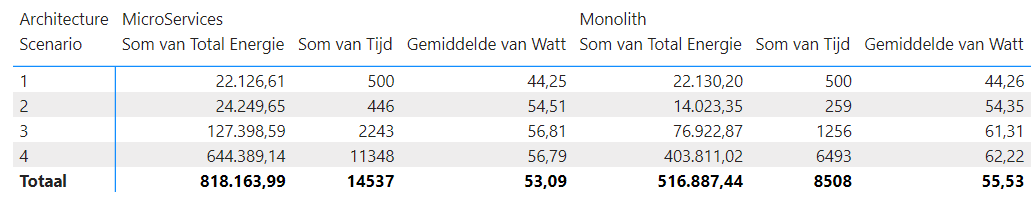
\includegraphics[scale=0.75]{apoc_totals_arch}
    \centering
    \caption{Voorbeeld scriptuitvoer testen PoC}
    \label{apoc_totals_arch}
\end{figure}

\begin{figure}[h!]
    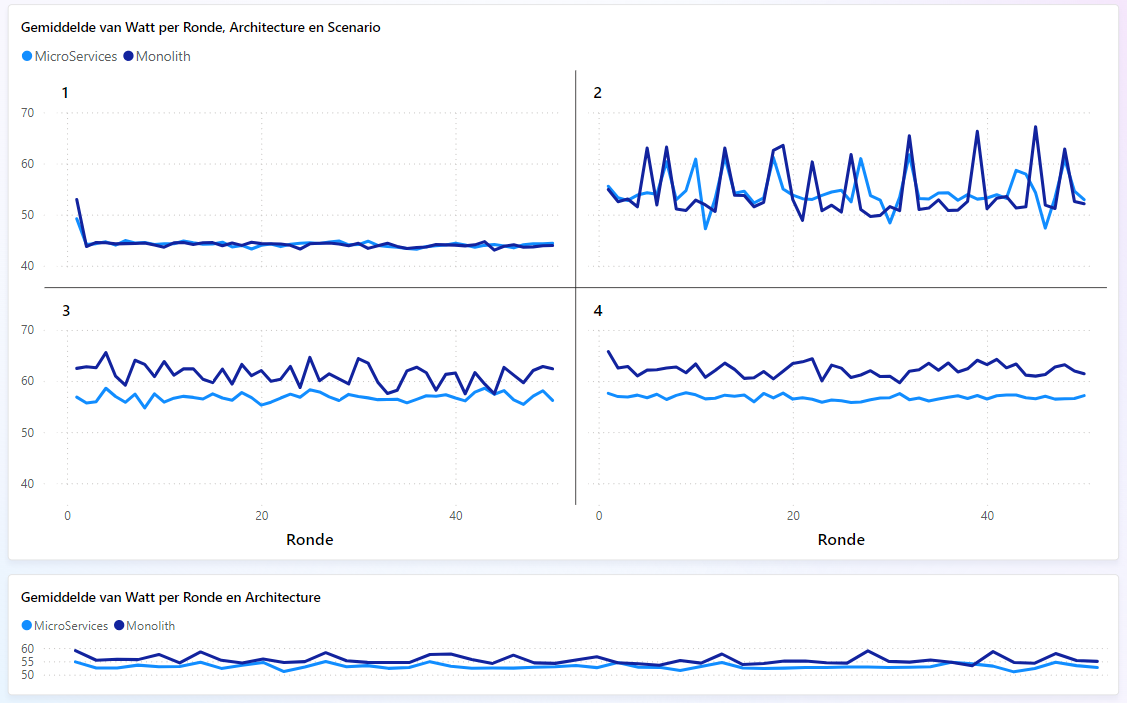
\includegraphics[scale=0.75]{apoc_avg_watt_arch_scen}
    \centering
    \caption{Voorbeeld scriptuitvoer testen PoC}
    \label{apoc_avg_watt_arch_scen}
\end{figure}

\begin{figure}[h!]
    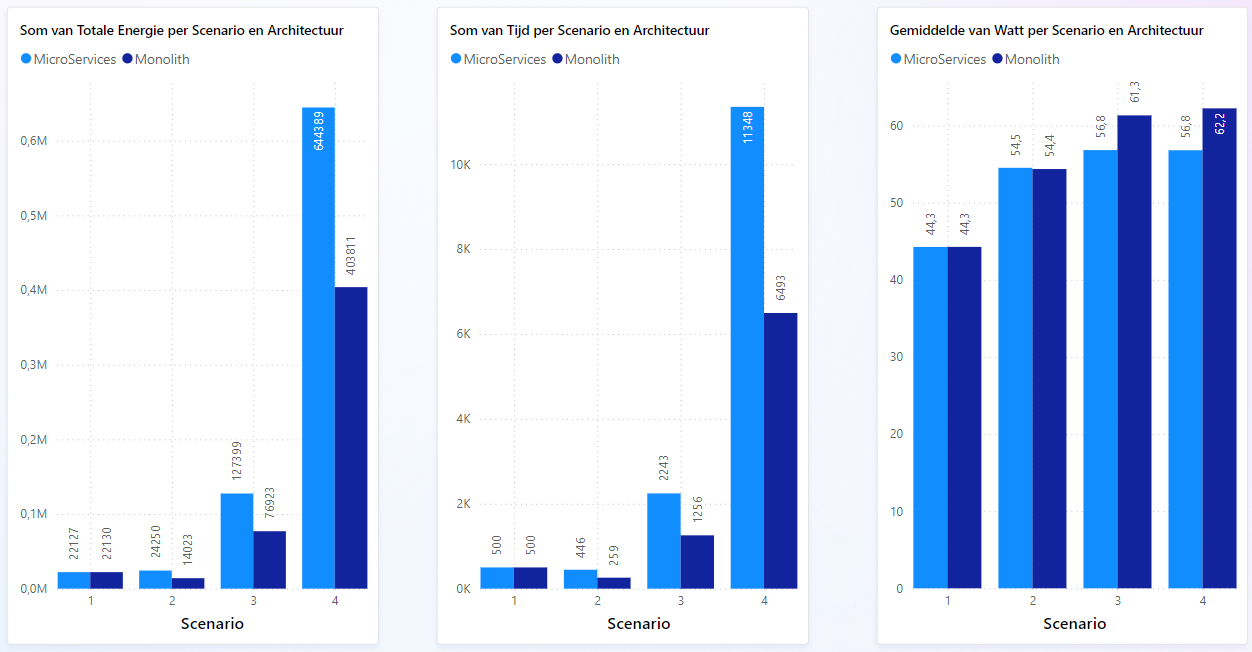
\includegraphics[scale=0.65]{apoc_3_graphs}
    \centering
    \caption{Voorbeeld scriptuitvoer testen PoC}
    \label{apoc_3_graphs}
\end{figure}

\begin{figure}[h!]
    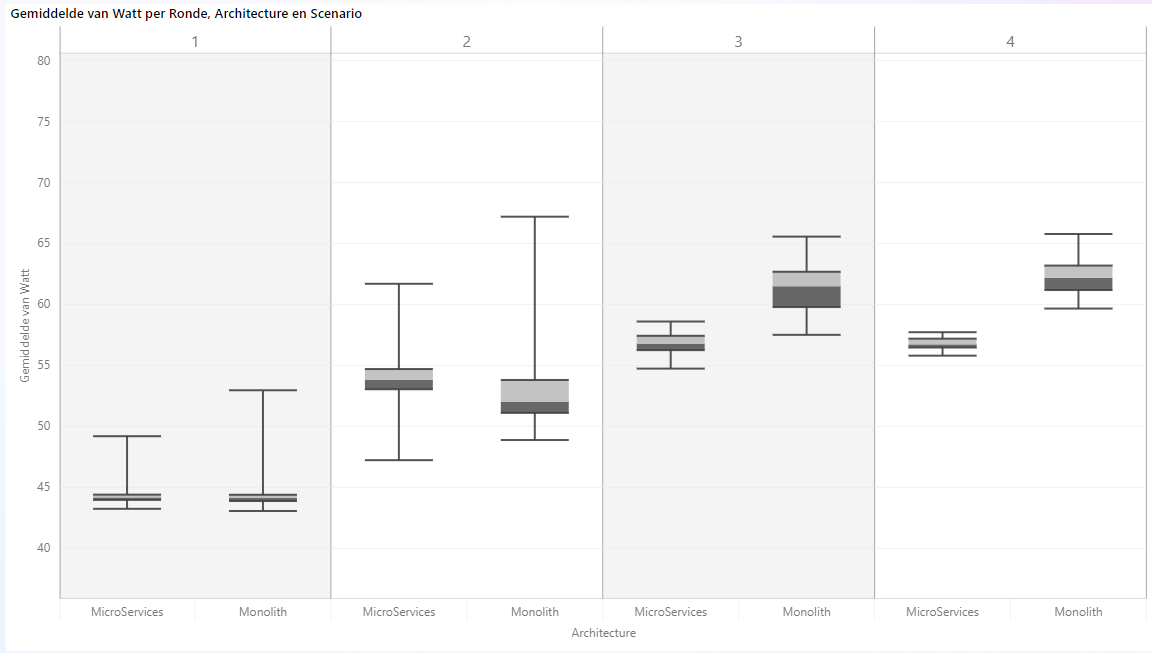
\includegraphics[scale=0.70]{apoc_avg_watt_deviation}
    \centering
    \caption{Voorbeeld scriptuitvoer testen PoC}
    \label{apoc_avg_watt_deviation}
\end{figure}

